\chapter{Marco teórico} \label{chap:contexto}            % ##   2. do Problema de Tabela Horária % Underfull \hbox (badness 2460)

Antes de prosseguirmos com o desenrolar deste trabalho, é adequado que primeiro definamos alguns parâmetros para o melhor entendimento do que está por vir.

% O Problema de Programação de Horários (Timetabling Problem) é um problema de grande relevância e amplamente estudado na área de Pesquisa Operacional. Um número significativo de trabalhos sobre esse problema foi publicado nos últimos anos e conferências regulares discutem o tema no meio científico [Splinder2010].
% Sânya
% O Problema de Programação de Horário Escolar pode ser generalizado como o escalonamento semanal das aulas em uma escola sem que professores e alunos tenham mais de uma aula ao mesmo tempo (estudantes são agrupados em turmas com os mesmos planos de aula). Já o Problema de Programação de Horário de Disciplinas em Universidades como o escalonamento semestral das aulas de um conjunto de disciplinas de uma universidade de modo a evitar colisão de horários (estudantes geralmente são considerados individualmente) [Paim__2010].
% Sânya

% Existem algumas ferramentas comerciais que prometem a geração automatizada de grades de horários, entretanto, sua utilização é pouco frequente uma vez que este tipo de problema incorre em necessidades específicas de um determinado curso, em detrimento das soluções genéricas existentes
% F. Vieira & H. Macedo, Scientia Plena 7, 039901 (2011) 

% O school timetabling possui uma quantidade de recursos menor, pois uma turma já possui uma sala especificada e seu grupo de alunos, em sua maioria, é predeterminado, o que faz com que a complexidade seja reduzida. Em problemas de course timetabling existe um grande conjunto de restrições: disciplinas de uma mesma turma podem ser alocadas em salas diferentes, cada disciplina é constituída por alunos de diversos cursos, professores possuem restrições de horário por desempenharem outras atividades na instituição, cada disciplina possui conjuntos de pré-requisitos que devem ser respeitados, entre outras.
% F. Vieira & H. Macedo, Scientia Plena 7, 039901 (2011) 

\section{Definição de termos} \label{sec:termos}              % ###  2.1

Ao longo dos anos de desenvolvimento acadêmico, diversos assuntos vão se aprofundando e se tornando mais específicos, assim, os estudiosos acabam cunhando novos termos que o auxiliam a desvencilhar as novas áreas específicas das suas áreas originárias. Porém, existe o potencial de que haja um crescimento desestruturado destes novos termos, assim vários termos diferentes podem se referir a um mesmo conceito, enquanto que um mesmo termo pode se referir a vários conceitos diferentes de acordo com o autor.

Segundo \citeonline{Wren1996}, podemos definir \textit{timetable} como uma estrutura que mostra quando que eventos ocorrerão, não havendo necessariamente a alocação de recursos. Vale ressaltar que este termo não tem seu uso limitado para os fins desta pesquisa, sendo também usado para problemas de alocação de enfermeiros, esportes, funcionários e transportes \cite{arratia-martinez_university_2021}. Entretanto, neste trabalho, abordaremos principalmente os termos relacionados ao que pode ser chamado de \textit{Educational Timetabling} (Ed-TT) \cite{Alencar2019}, que é o que tende a envolver um conjunto específico de recursos relacionados à educação.

\citeonline{Wren1996} também define os conceitos para \textit{class timetable}, \textit{university examination timetable} e \textit{university class timetable}, tendo relevância apenas o último, que considera a disponibilidade de professores e salas, a quantidade de alunos e os requisitos que determinada disciplina exige.

Assim como feito por \citeonline{Wren1996}, definiremos os conceitos dos termos que serão usados ao longo deste trabalho. Sendo assim, usaremos a definição do termo \textit{university class timetable} de forma simplificada, sendo chamada apenas de \textit{timetable}, ``grade horária'' ou ``tabela horária''.

% Sânya fala sobre International Timetabling Competition

Aqui, visto que uma solução final envolverá várias dimensões (Professores $\times$ Disciplinas $\times$ Sala $\times$ Alunos $\times$ Horários $\times$ Dias), consideraremos \textit{timetable} como esse pacote de valores distribuídos em uma só estrutura. Para que esses valores sejam distribuídos, daremos o nome de \textbf{alocação} ao ato de criar qualquer relação entre as dimensões. Como a relação de horários e dias será considerada fixa, a \textbf{alocação} se referirá à atribuição como a de professores a disciplinas, disciplinas a salas, disciplinas a um determinado padrão de dias e horários, etc.

Para que esta alocação ocorra, é necessário atender a certos critérios, e aí entra o ``problema de organização de grade horária'', também chamado de \textit{timetabling problem}. Esta é uma subcategoria do \textbf{problema de agendamento} (\textit{scheduling Optimization Problem}) \cite{Alencar2019} que por sua vez é definido por \citeonline{Wren1996} como sendo:

\begin{quote}\footnotesize
  Resolver problemas práticos relacionados à alocação, sujeito a restrições, de recursos a objetos sendo colocados no espaço-tempo, usando ou desenvolvendo quaisquer ferramentas que possam ser apropriadas. Os problemas irão frequentemente se relacionar à satisfação de certos objetivos.
\end{quote}

Outro termo relevante a se pontuar são as \textit{hard and soft constraints} que podemos chamar de restrições rígidas e flexíveis. \citeonline{Alencar2019} as define dizendo que as restrições rígidas são de atendimento obrigatório, enquanto as restrições flexíveis são opcionais, mas convenientes para melhorar a qualidade da solução obtida.

Exemplo de restrição rígida: nem professores nem alunos podem ser alocados simultaneamente a duas salas ou disciplinas simultaneamente. Uma solução que viole esta restrição se torna automaticamente inviável.

Exemplo de restrição flexível: professor J. prefere não dar aulas nas tardes de sexta-feira, e prefere dar aula nas manhãs da segunda-feira. Uma solução que viole esta restrição não se torna inviável, porém tende a ter menos valor neste critério do que uma solução que siga as preferências definidas.

Alguns outros termos similares a este campo de pesquisa encontrados na literatura são \textit{periodic event scheduling problem}, \textit{timetable scheduling}, \textit{class scheduling}, \textit{student scheduling}, \textit{university course timetabling}, dentre outros.

\section{Métodos de resolução} \label{sec:resolucao}          % ###  2.2

% - O problema de timetabling   a
%  - Origem                    a
%  - Repartições               a
%  - Escopo maior              a
%    - Scheduling              a
%  - Escopo menor              a
%    - Exam                    a
%    - Class                   a
% - TT
%  - Soluções
%  - Desafios
%  - Diversas formas de resolução
%    - Graph Coloring
%    - Heurísticas
%    - Meta-heurísticas
%    - IA
%    - etc.
% - Visualização de informações
%  - Benefícios
%  - Motivações
%  - Relação com timetabling
% - Problema geral a ser resolvido
%  - Multi dimensionalidade
%    - Professores
%    - Alunos
%    - Salas
%    - Departamentos
%      - Preferências
%      - Concorrências
%  - Otimalidade
%  - Erros humanos
%  - Número de possibilidades
%  - Interface intuitiva e relevante é um desafio com poucos estudos nos últimos anos
% - Problemas específicos
%  - Regras específicas
%  - Prioridades diferentes
%  - estrutura organizacional semi-exclusiva

% Pesquisar posteriormente sobre imagens que ilustrem bem as diferentes sub categorias de scheduling

Existem diversas implementações já realizadas, utilizando uma miríade de métodos. Em seu trabalho, \citeonline{miranda_udpskeduler_2012} informam sobre diversos sistemas baseados em computador para auxiliar na tarefa de agendamento. \citeonline{miranda_udpskeduler_2012} também citam um dos métodos de resolução como sendo o \textbf{modelo de programação inteira} e \textbf{heurísticas}.

Outros trabalhos buscaram condensar em forma de tabela as informações encontradas. Abaixo estão dispostas algumas das tabelas encontradas durante o estudo bibliográfico e que foram elaboradas por diversos autores.

Na \autoref{fig:Desenvolvimento}, \citeonline{alegre_desenvolvimento_2012} traça a relação entre os diversos autores, ano de sua publicação e seu país de origem com os dados encontrados em seus trabalhos quanto aos parâmetros utilizados na elaboração da grade horária, quão grandes eram cada um de seus parâmetros, quanto tempo foi necessário para achar uma solução e quais foram as técnicas utilizadas.

% Entender o que está dando errado aqui depois

\begin{CenteredFigure} \caption{Resumo de trabalhos, parâmetros, dimensões, tempo e técnicas.} \label{fig:Desenvolvimento}
  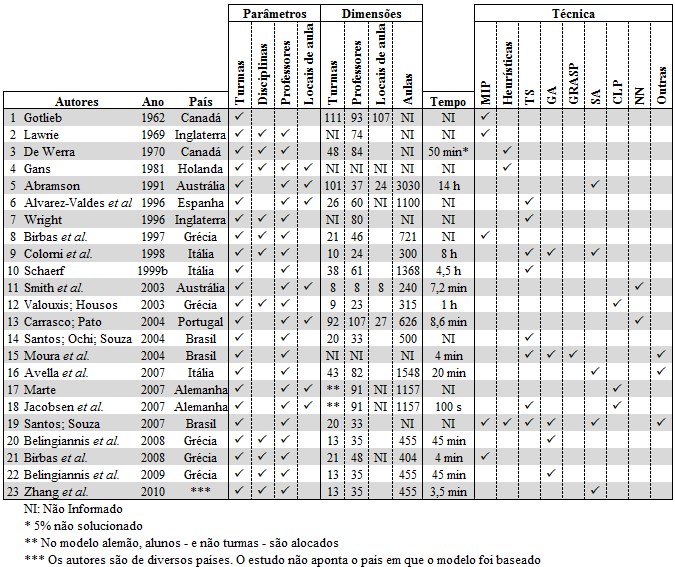
\includegraphics[width=\textwidth]{files/img/2.02!2-contexto/Desenvolvimento}
  \legend{Fonte: \citeonline{alegre_desenvolvimento_2012}}
\end{CenteredFigure}    % Desenvolvimento

Na \autoref{fig:University}, \citeonline{arratia-martinez_university_2021}, apresentam uma comparação similar à anterior, porém não separada em categorias, apenas categorizando entre verdadeiro e falso algumas características como alocação de salas, professores, nível institucional e método exato ou inexato.

\begin{CenteredFigure} \caption{Comparação entre artigos que solucionam o problema de grade horária} \label{fig:University}
  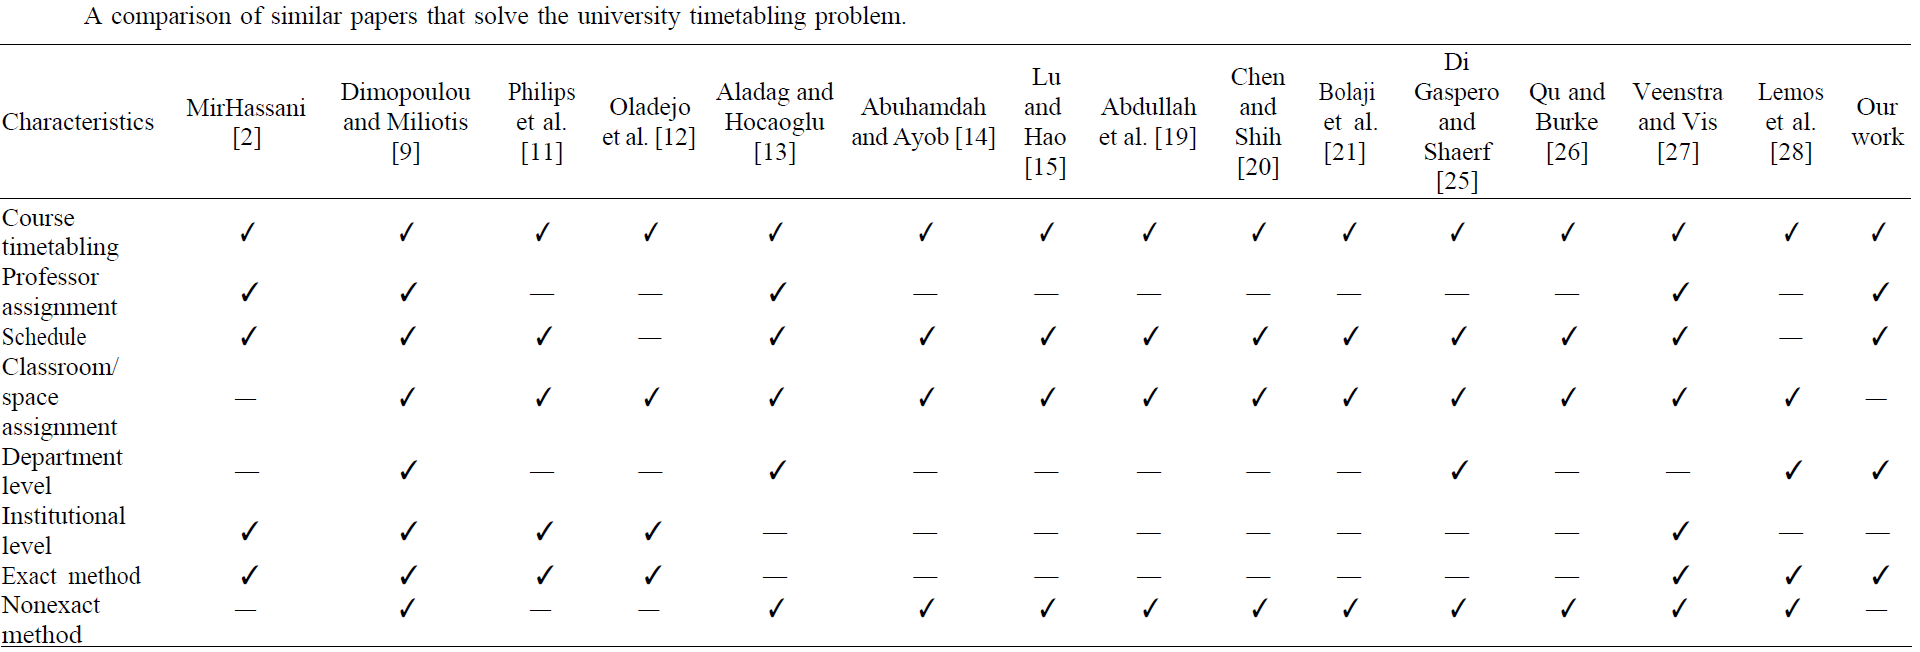
\includegraphics[width=\textwidth]{files/img/2.02!2-contexto/University}
  \legend{Fonte: \citeonline{arratia-martinez_university_2021} - editado}
\end{CenteredFigure}    % University

Na \autoref{fig:Visualization}, \citeonline{Alencar2019} exploram uma categoria mais específica do problema, que é a característica da interatividade das interfaces desenvolvidas. Este apresenta características qualitativas quanto aos métodos, os dados dispostos, as técnicas de interação e o método utilizado para solucionar o problema de grade horária educacional. Nesta figura, os autores usam ``Y'' para simbolizar ``Sim'', ``N'' para ``Não'' e ``-'' para ``Inconclusivo''.

\begin{CenteredFigure} \caption{Análise de publicações aceitas} \label{fig:Visualization}
  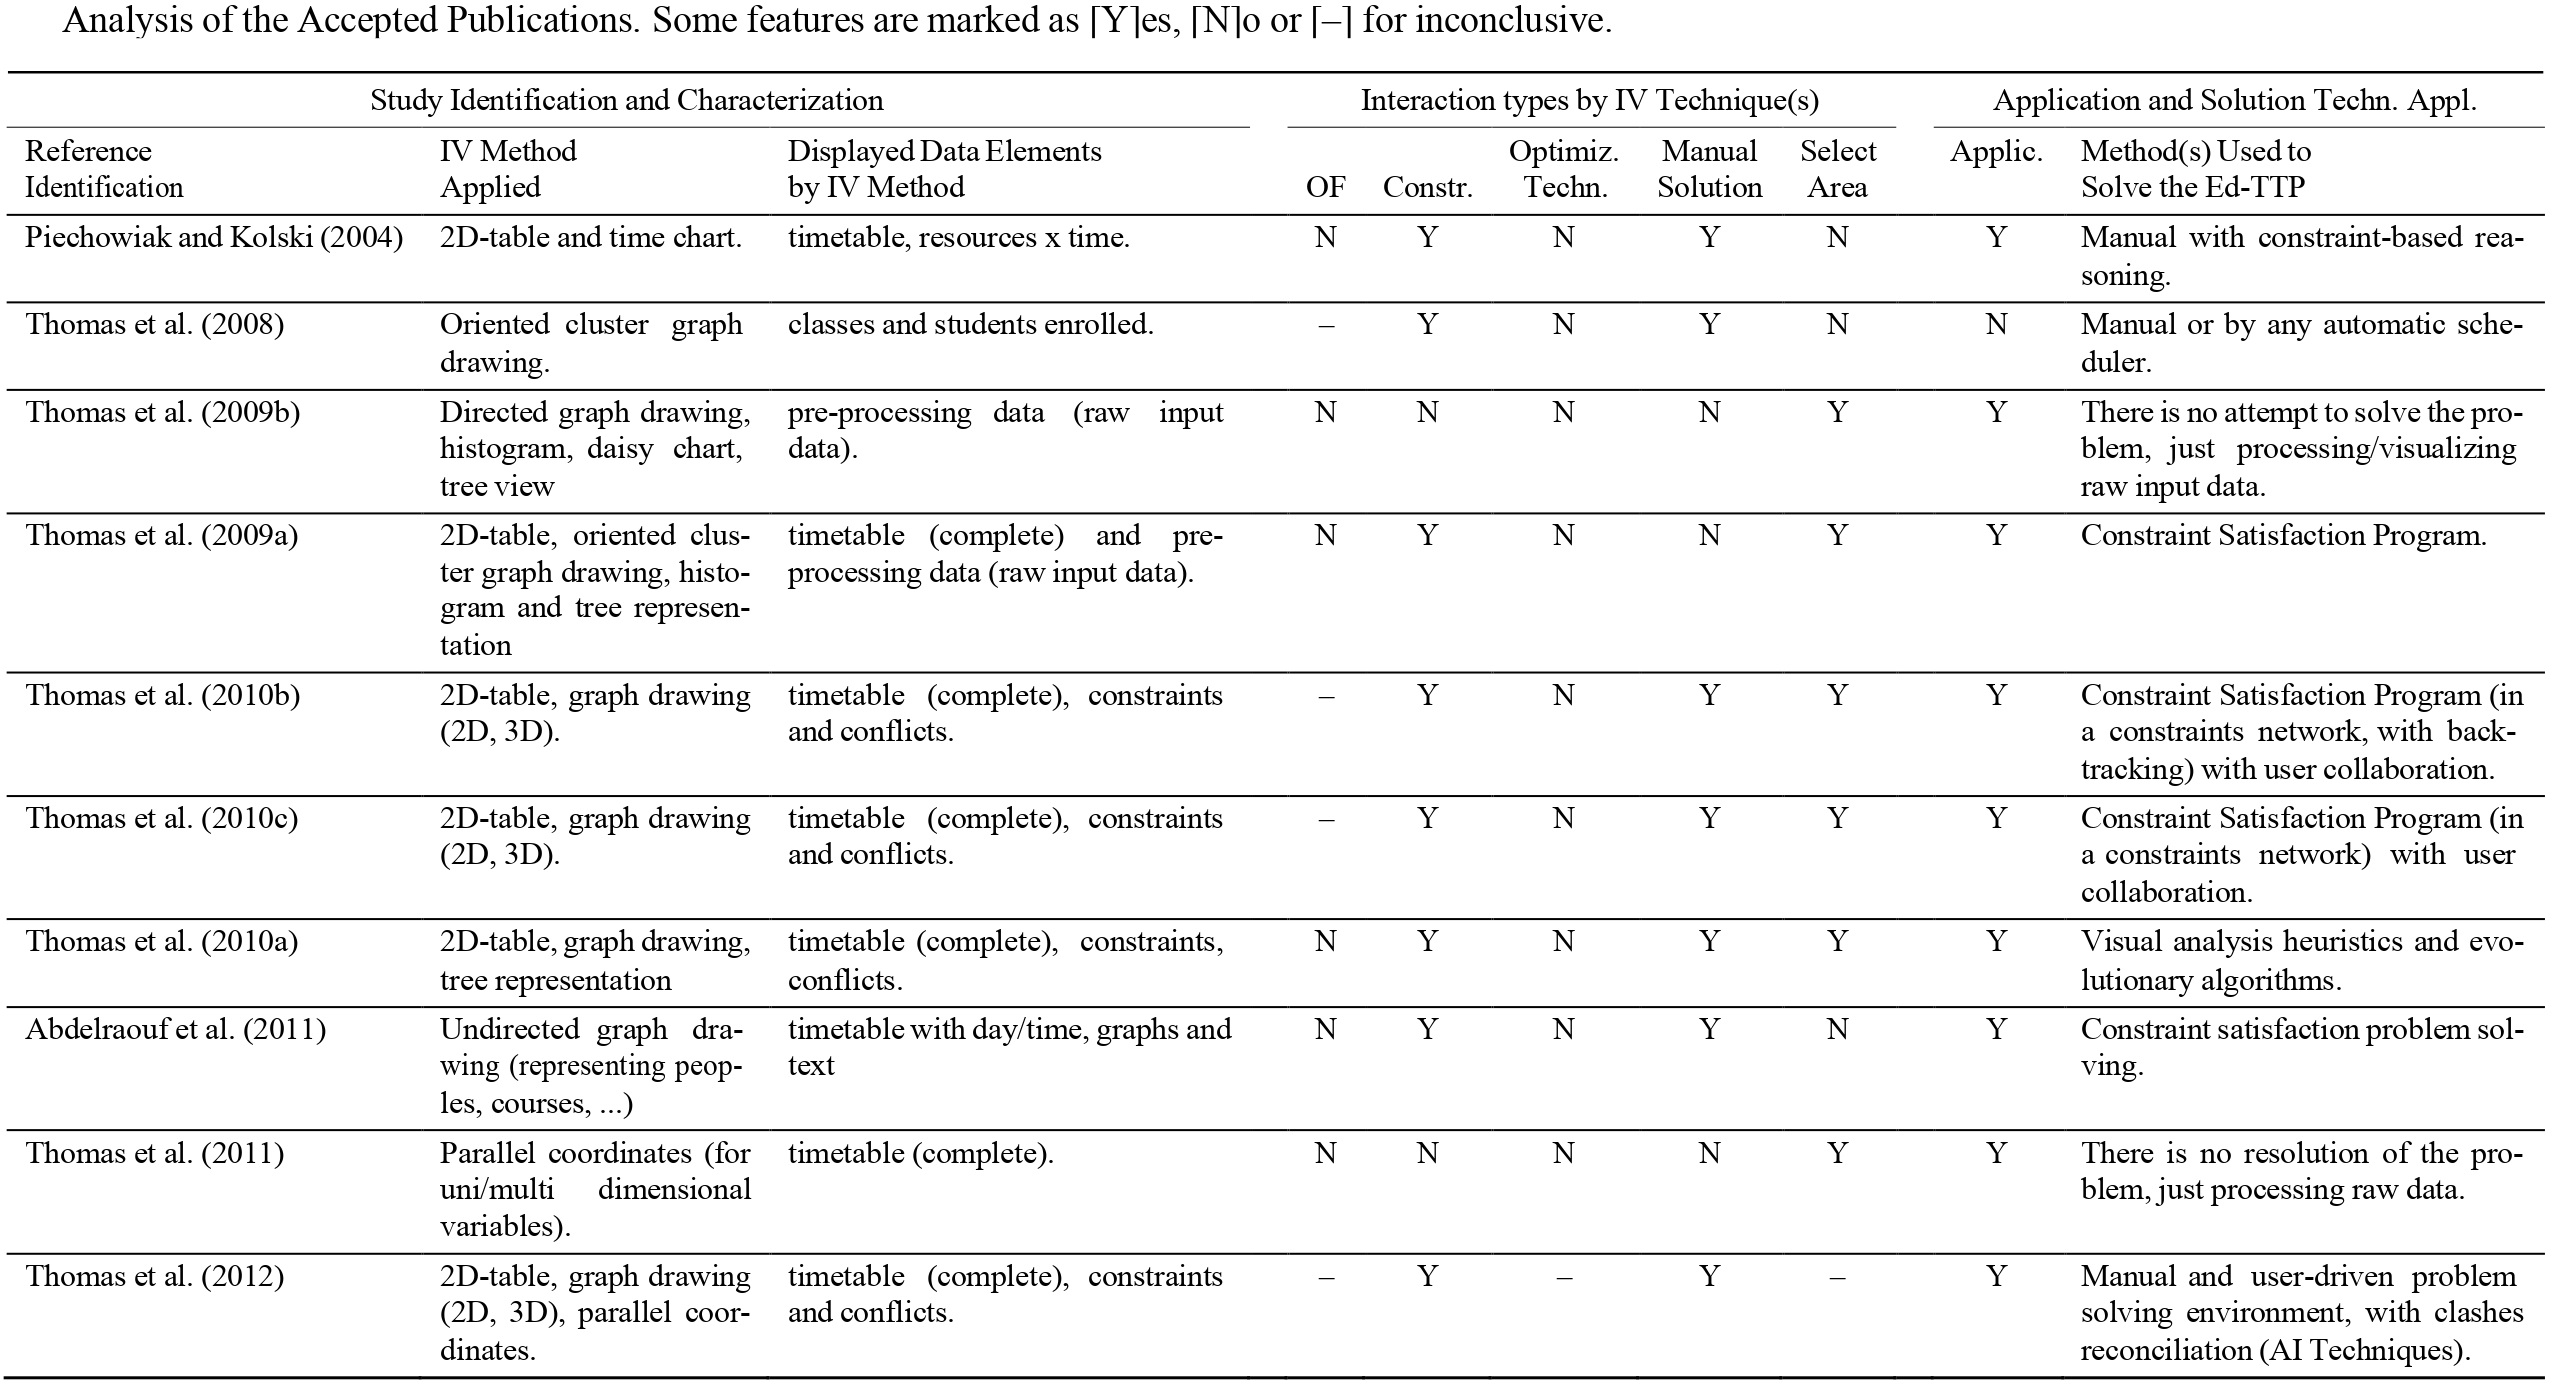
\includegraphics[width=\textwidth]{files/img/2.02!2-contexto/Visualization}
  \legend{Fonte: \citeonline{Alencar2019} - editado}
\end{CenteredFigure}    % Visualization

\section{Desafios recorrentes} \label{sec:desafios}           % ###  2.3

Apesar da vasta quantidade de trabalhos realizados com este fim, o \textit{Timetabling Problem} segue sendo uma área sem uma solução definitiva.

\citeonline{Murray2007} trazem a questão da modelagem como um dos maiores obstáculos. À medida em que a complexidade aumenta, se torna cada vez mais difícil desenvolver uma solução efetiva. Assim fazendo com que a solução para uma universidade possa não ter utilidade para outras, ou até mesmo não seja capaz de lidar com todos os problemas de uma mesma universidade.

Apesar do contrafluxo encontrado na resolução desse problema, \citeonline{Murray2007} citam que, apesar da complexidade, é sim possível desenvolver soluções que tenham uso prático, mesmo que não seja um processo fácil. As ferramentas existem e estão disponíveis. Restando então considerar e resolver as preocupações dos usuários às questões, visto que as técnicas de resolução já se encontram vastamente documentadas.

Com isso, entramos também no ramo da Interação Homem-Máquina, ramo abordado por \citeonline{Andre2018} que visaram em seu desenvolvimento a criação de uma interface focada no usuário. Assim minimizando o atrito na abordagem desse problema complexo. Também sendo área de enfoque de \citeonline{Alencar2019} em sua revisão literária

\section{\textit{Timetabling} na UENF} \label{sec:anteriores} % ###  2.4

Este trabalho não se mostra desprovido de histórico na tentativa de resolução do mesmo problema. Sânya e Ricardo, ambos estudantes de Ciência da Computação da UENF, já realizaram trabalhos com o mesmo fim, porém com abordagens diferentes da atual proposta.

Tendo vista que atualmente o problema de Programação Horária da UENF ainda perdura, podemos considerar que embora os trabalhos anteriores tenham se mostrado importantes ao pavimentar o caminho em direção à resolução da problemática disposta, as soluções ótimas encontradas por ambos, embora ótimas para a modelagem proposta, não se mostraram ótimas para a realidade da universidade.

Abaixo são listados os trabalhos anteriores e suas respectivas abordagens, bem como os apontamentos do que se mostrou inviável para a realidade da universidade.

\subsection{Sânya Carvalho dos Santos} \label{subsec:sanya}   % #### 2.4.1

Em seu trabalho, \citeonline{Sanya2013} aborda o problema de Programação de Horários de Disciplinas em Universidades, tendo como foco o curso de Ciência da Computação da UENF. Sua abordagem foi a de desenvolver um software que fosse capaz de gerar uma grade horária ótima para o curso, levando em conta as restrições impostas pelo curso. Para isso, Sânya explicou diversos métodos possíveis para se alcançar a solução desejada, passando inicialmente pelos métodos construtivos, seguido de métodos refinamento, podendo essas heurísticas serem utilizadas em conjunto com meta-heurísticas.

Por fim, utilizou uma heurística que consistia em respeitar a uma matriz de preferência para a distribuição das disciplinas. Seguindo com o uso do \textit{Simulated Annealing} para a otimização da solução inicial.

\subsection{Ricardo Couto da Silveira} \label{subsec:ricardo} % #### 2.4.2

Em seu trabalho, \citeonline{Ricardo2014} aborda também o Problema de Programação de Horários (PPH) em instituições de ensino superior. Ele explora os diversos métodos heurísticos para resolução deste problema que visa encontrar a alocação ótima dos horários em suas grades. Ele teve como objetivo de seu trabalho a implementação de um software que fosse capaz de resolver o PPH do curso de Ciência da Computação da UENF, utilizando os métodos heurísticos Construção Gulosa e Busca Local e os métodos metaheurísticos \textit{Simulated Annealing} e Busca Tabu. Para este fim, ele utilizou a linguagem de programação C para a implementação dos métodos e a linguagem de programação Java para a implementação da interface gráfica do software. Com isso conseguiu elaborar uma ferramenta automatizada para a geração de quadros de horários, alocando aulas e professores em dias e horários disponíveis na semana.

Ele descreve também como possibilidade de trabalho futuro o aperfeiçoamento do banco de dados da ferramenta desenvolvida para que se possa armazenar mais informações pertinentes ao problema, para que o usuário possa realizar modificações no quadro de horários, sendo guiado pelo retorno do Software que informa a viabilidade da alteração, assim gerando maior flexibilidade à aplicação.

\subsection{Divergências} \label{subsec:divergencias}         % #### 2.4.3

Embora ambos os trabalhos tenham sido de grande valia ao rumarem na direção de uma solução para este amplo e complexo problema, percebe-se que o problema que buscaram solucionar ainda se encontra em aberto. Não tendo suas ferramentas alçado voos altos o suficiente para que se tornassem soluções definitivas para o problema no contexto da UENF.

\subsubsection*{Sânya} \label{subsubsec:sanya} % ##### 2.4.1.1

É dito por \citeonline{Sanya2013} que ``[...] Como na UENF a tarefa de distribuição de sala não varia muito a cada período, sendo feito separadamente por cada centro [...]''. Embora possamos entender o conceito de ``variar muito'' como subjetivo, considerando que mesmo ao longo de um mesmo semestre existem realocações de salas e professores dentro do contexto de um mesmo Centro, podemos entender que a realidade da UENF é de fato muito dinâmica, não se encaixando completamente na solução de alocação única inicial de salas e professores.

Pode-se alegar que tratar da variabilidade de alocações de salas de um mesmo Centro foge do escopo do trabalho, porém, para que o coordenador da Computação tenha fácil acesso aos dados de alocação de salas disponíveis, faz-se necessário que seu uso esteja compartilhado com o Diretor do Centro de Ciência e Tecnologia (CCT), visto que este é o responsável pela alocação de salas de todos os cursos do CCT.

Em outro segmento ela diz que ``[...] as aulas que necessitam de salas com recursos especiais são geralmente já preestabelecidas, não há necessidade de automatizar esta tarefa de distribuição de salas'', mas a realidade é que embora algumas disciplinas tenham suas salas pré-estabelecidas, não são todas as disciplinas que possuem esta característica, isso não significa necessariamente que esta alocação é a mais adequada para a mesma. Então, todas as salas, mesmo que inicialmente pré-estabelecidas, devem estar passíveis de mudanças, mas com possibilidade de se fixar.

Ela diz também que ``Outra tarefa que no presente cenário do curso de Ciência da Computação não viabiliza algum tipo de automatização é a distribuição de professores, pois além de um número muito pequeno destes, não há muitas alternativas de mudanças de suas respectivas disciplinas.''

Quanto à distribuição de professores, a realidade do curso de Ciência da Computação segue a mesma da que foi apontada por \citeonline{Sanya2013}. Entretanto, cada professor tem sua própria gama de disciplinas que se dispõe a ministrar, e a coordenação tende a distribuí-los de acordo com sua preferência. Entretanto, como a demanda dos alunos não se mostra linear como foi estudado, é possível que a distribuição de professores seja feita de forma mais eficiente, considerando a demanda dos alunos, ainda que não se descartem suas preferências pessoais.

Sânya apresenta em seu trabalho uma série de requisitos essenciais e não essenciais para a resolução do problema. Porém, alguns deles não se mostram condizentes com a realidade da universidade. São eles:

\begin{quote}\footnotesize
  \begin{itemize}
    \item Requisitos essenciais, ou seja, obrigatórios:
          \begin{itemize}
            \item \textbf{RE1} - Um professor não pode lecionar aula em duas turmas diferentes no mesmo horário.
            \item \textbf{RE2} - Uma turma não pode ter aula em duas disciplinas no mesmo horário.
          \end{itemize}
    \item Requisitos não essenciais, de qualidade:
          \begin{itemize}
            \item \textbf{RNE1} - O ideal é que existam no máximo duas aulas consecutivas da mesma disciplina.
            \item \textbf{RNE2} - Não devem haver mais de duas aulas da mesma disciplina em um dia.
            \item \textbf{RNE3} - Não preencher os horários de 12h às 14h, pois se trata de horário de almoço.
            \item \textbf{RNE4} - Os professores associados, por terem exclusividade com a instituição, preferem espalhar os horários das aulas dadas, e não acumular todas no mesmo dia.
            \item \textbf{RNE5} - Os professores contratados, por outro lado, preferem que suas aulas sejam alocadas num mesmo dia, ou no menor número de dias possíveis.
          \end{itemize}
  \end{itemize}
\end{quote}

Quanto à citada RE2, a limitação deveria ser mais criteriosa, e se tratando de um requisito não essencial, pois, o conceito de turma é dado pela junção de estudantes que cursam a mesma disciplina, ministrada por um mesmo professor, em um mesmo semestre. Mas em seu trabalho, Sânya considera o conceito de turma como sendo o conjunto de estudantes que ingressaram em um mesmo ano, independente da consideração da existência de repetentes e de suas escolhas pessoais de inscrição.

\textbf{RNE1}, \textbf{RNE2} e \textbf{RNE3}: todas elas não consideram a existência de disciplinas que necessitam de um total de cinco tempos de aula semanais, sendo elas regularmente divididas em dois períodos, um de duas horas e outro de três horas. Que, em situações de necessidades, como é visto na entrevista com o diretor do CCT, acaba sim sendo necessário que se aloque em período de almoço.

\textbf{RNE4} e \textbf{RNE5}: embora estejam direcionadas corretamente, ainda assim não engloba casos de preferência pessoal de cada um dos professores citados. Como por exemplo a possibilidade de não se ministrar aulas em determinados dias da semana por motivos religiosos, seja por parte do quadro permanente, quanto de professores associados.

Outra considerável divergência entre o modelo e a realidade é a definição de que a cada semestre contém apenas 5 turmas de computação. Sendo estas compostas pelos estudantes ingressantes de 5 anos consecutivos, caso este que não se aplica à realidade da universidade, visto que a quantidade de turmas varia de acordo com a demanda semestral, que não necessariamente condiz com todos os estudantes ingressantes de um mesmo ano.

Por fim, Sânya não considera a possibilidade de alocação de professores em mais de uma disciplina, o que é uma realidade na universidade, visto que alguns professores ministram aulas em mais de um curso, e em mais de uma disciplina.

\subsubsection*{Ricardo} \label{subsubsec:ricardo} % ##### 2.4.1.2

\citeonline{Ricardo2014}, em seu trabalho, apresenta alguns conceitos que se mostraram limitantes em sua modelagem conceitual do problema na UENF. Em sua monografia, ele aborda as turmas como sendo compostas por alunos que ingressaram no mesmo ano, independente de suas escolhas, da demanda, e de possíveis defasagens na progressão do curso. O que não se mostra condizente com a realidade da universidade atualmente, então, mesmo que em 2014, quando o trabalho foi realizado, a realidade fosse esta, não se mostra condizente com a realidade atual, havendo então a necessidade de uma reformulação conceitual.

Ele, assim com \citeonline{Sanya2013}, também não considera a possibilidade de alocação de professores em mais de uma disciplina, múltiplas turmas de uma mesma disciplina, assim como não lida com a distribuição das salas. Ele também considera algumas disciplinas estão fixas, mesmo que pudessem sim ser modificadas por seu responsável, o Diretor do CCT.

Por fim, podemos citar um outro ponto que é a busca pela eficiência e baixo custo de tempo dos métodos utilizados. O que se mostra como ponto positivo, entretanto, mesmo com tamanha eficiência ainda peca em atingir a praticabilidade da solução.

\subsubsection*{Parecer geral das divergências} \label{subsubsec:divergencias} % ##### 2.4.1.3

O entendimento das falhas passadas em se encontrar uma solução prática ao problema de Programação de Horários da UENF é de suma importância para que se possa evitar que os mesmos erros sejam cometidos novamente. Assim, é necessário que se tenha em mente que a realidade da universidade é dinâmica, e que a solução deve ser capaz de se adaptar a esta dinamicidade.

Vale-se também relembrar o que é dito por \citeonline{Murray2007} que citam em seu trabalho justamente sobre a complexidade presente na modelagem do problema.

\section{Exemplo de erros humanos} \label{sec:erros}          % ###  2.5

Dada a grande quantidade de variáveis interconectadas e as características específicas de cada instituição \cite{miranda_udpskeduler_2012}, a organização destas informações buscando a melhor solução possível apresenta-se como um desafio. Principalmente se considerarmos que esta solução é, muitas vezes, buscada manualmente, estando também passível de erros humanos como ilustram a \autoref{fig:Academico} e \autoref{fig:CCT}.

\begin{MyCenteredFigure} \caption{Disciplina atribuída no sistema acadêmico à determinada hora e local} \label{fig:Academico}
  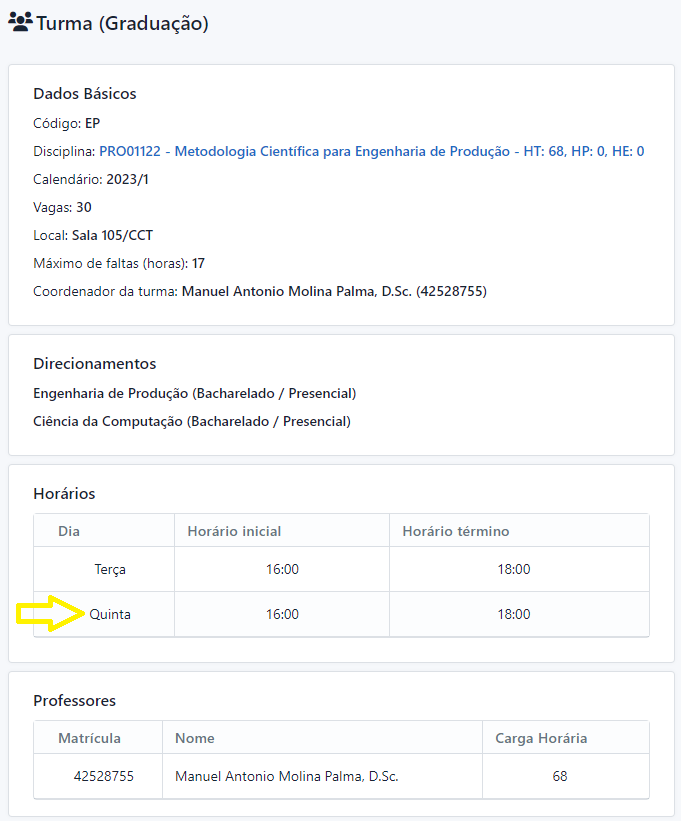
\includegraphics[width=\textwidth]{files/img/2.02!3-organizacao/2.02!3.1.5-erros/Metodologia-Quinta}
\end{MyCenteredFigure}    % Imagem acadêmico

\begin{MyCenteredFigure} \caption{Falha de alocação na grade horária do CCT de 2023.1} \label{fig:CCT}
  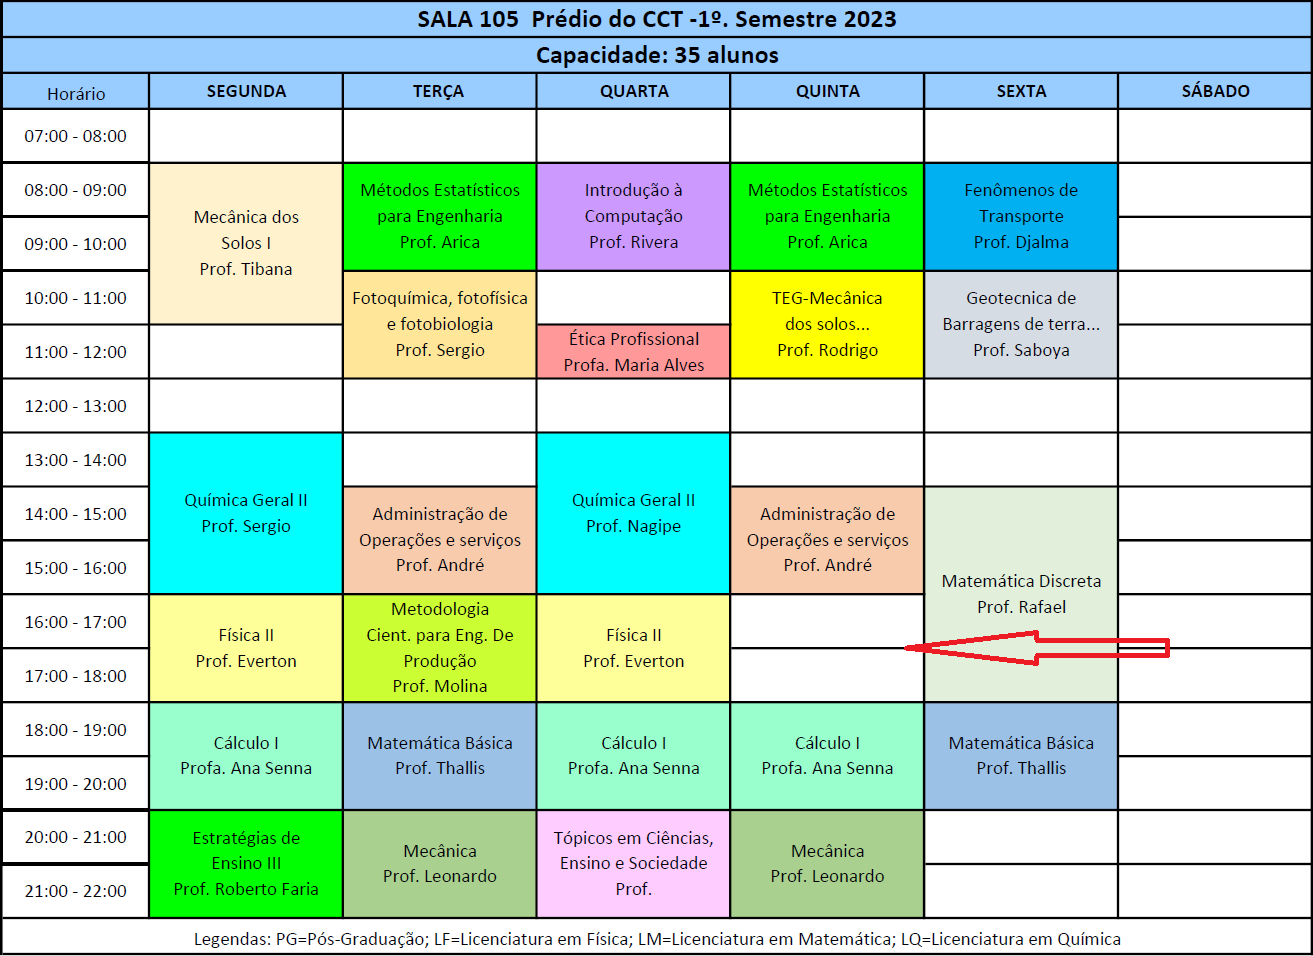
\includegraphics[width=\textwidth]{files/img/2.02!3-organizacao/2.02!3.1.5-erros/Aulas-CCT-105-2023_1}
\end{MyCenteredFigure}    % Imagem representando o erro humano na alocação de salas

Nestas imagens, fica exemplificado um dos possíveis problemas que podem ocorrer durante a criação de grades horárias, que é, mesmo quando uma seção da universidade (o Sistema Acadêmico, ilustrado pela \autoref{fig:Academico}) aloca uma turma a uma determinada sala, outra seção da mesma instituição (o Centro de Ciência e Tecnologia, ilustrado pela \autoref{fig:CCT}) pode não estar ciente do mesmo, ou mesmo estando ciente pode acabar não delimitando aquela lacuna de tempo como ocupada, assim estando passível de uma segunda alocação naquele período de tempo naquela sala, assim gerando problemas.
